	\paragraph{QuizziPedia::Front-End::AppRun}
		
		\label{QuizziPedia::Front-End::AppRun}
		
		\begin{figure}[ht]
			\centering
			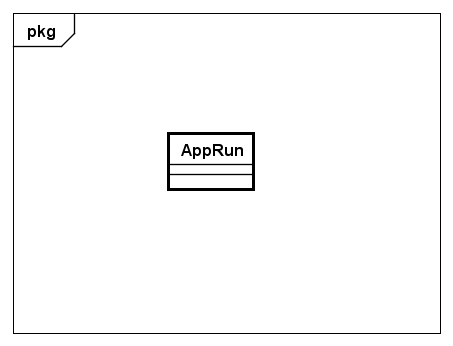
\includegraphics[scale=0.45,keepaspectratio]{UML/Classi/Front-End/QuizziPedia_Front-end_AppRun.png}
			\caption{QuizziPedia::Front-End::AppRun}
		\end{figure} \FloatBarrier
		
		\begin{itemize}
			\item \textbf{Descrizione}: classe che verifica se l'utente sia autenticato e che abbia le giuste autorizzazioni per la pagina in cui si trova;
			\item \textbf{Utilizzo}: viene utilizzata per verificare che l’utente sia autenticato e che abbia la giusta autorizzazione per la pagina in cui si trova;
			\item \textbf{Relazioni con altre classi}: 
			\begin{itemize}
				\item \textbf{IN} \texttt{LangService}: questa classe permette di gestire la lingua nella quale si è scelto di utilizzare l'applicazione;
				\item \textbf{IN} \texttt{LangModel}: rappresenta le informazioni per la giusta traduzione dell'applicazione;
				\item \textbf{IN} \texttt{UserDetailsModel}: rappresenta un utente. Contiene tutte le informazioni necessarie alla presentazione del contenuto di un utente sia nella visualizzazione che nella gestione di un profilo;
				\item \textbf{IN} \texttt{AuthService}: questa classe permette di gestire la registrazione e l'autenticazione di un utente.
			\end{itemize}
			\item \textbf{Attributi}: 
			\begin{itemize}
				\item \texttt{-} \texttt{\$scope: \$scope} \\
				Campo dati contenente un riferimento all'oggetto \$scope creato da \textit{Angular\ped{G}};
				\item \texttt{-} \texttt{\$rootScope: \$rootScope} \\
				Campo dati contenente il riferimento all'oggetto globale \$rootScope creato da \textit{Angular\ped{G}};
				\item \texttt{-} \texttt{\$location: \$location} \\
				Campo dati contenente un riferimento al servizio creato da \textit{Angular\ped{G}} che permette di accedere alla barra degli indirizzi del \textit{browser\ped{G}}, i cambiamenti all'URL nella barra degli indirizzi si riflettono in questo oggetto e viceversa;
				\item \texttt{-} \texttt{\$mdDialog: \$mdDialog} \\
				Campo dati contenente un riferimento al servizio della libreria \textit{Material for Angular\ped{G}} che permette di creare delle componenti a pop-up;
				\item \texttt{-} \texttt{AuthService: AuthService} \\
				Campo dati contenente un riferimento al servizio che si occupa della gestione delle informazioni legate all'autenticazione;
				\item \texttt{+} \texttt{userOnScope: UserDetailsModelView} \\
				Oggetto di tipo \texttt{UserDetailsModelView}. Rappresenta l'oggetto dell'utente autenticato all'interno dello \texttt{\$rootScope};
				\item \texttt{-} \texttt{user: UserDetailsModel} \\
				Oggetto di tipo \texttt{UserDetailsModel}. Rappresenta l'oggetto dell'utente autenticato;
				\item \texttt{+} \texttt{lang: LangModel} \\
				Oggetto di tipo \texttt{LangModel}. Rappresenta l'oggetto contenente la giusta traduzione del template delle pagine.
			\end{itemize}
			\item \textbf{Metodi}: 
			\begin{itemize}
				\item \texttt{+} \texttt{AppRun(\$scope: \$scope, \$rootScope: \$rootScope, \$location: \$location, \$mdDialog: \$mdDialog, AuthService: AuthService, UserDetailsModel: \\UserDetailsModel)} \\
				Metodo costruttore della classe. Recupera dopo il login tutte le informazioni dell'utente. Recupera anche da  \\
				\textbf{Parametri}:
				\begin{itemize}
					\item \texttt{\$scope: \$scope} \\
					Parametro contenente un riferimento all’oggetto \$scope creato da \textit{Angular\ped{G}}. Viene utilizzato come mezzo di comunicazione tra il controller e la view. Contiene gli oggetti che definiscono il viewmodel e il model dell’applicazione;
					\item \texttt{\$rootScope: \$rootScope} \\
					Parametro contenente il riferimento all'oggetto globale \$rootScope creato da \textit{Angular\ped{G}};
					\item \texttt{\$location: \$location} \\
					Parametro contenente un riferimento al servizio creato da \textit{Angular\ped{G}} che permette di accedere alla barra degli indirizzi del \textit{browser\ped{G}}, i cambiamenti all’URL nella barra degli indirizzi si riflettono in questo oggetto e viceversa;
					\item \texttt{\$mdDialog: \$mdDialog} \\
					Parametro contenente un riferimento al servizio della libreria \textit{Material for Angular\ped{G}} che permette di creare delle componenti a pop-up;
					\item \texttt{AuthService: AuthService} \\
					Parametro contenente un riferimento al servizio che si occupa della gestione delle informazioni legate all’autenticazione;
					\item \texttt{UserDetailsModel: UserDetailsModel} \\
					Parametro contenente un riferimento alla classe per poter istanziare un oggetto di tipo \texttt{UserDetailsModel}.
				\end{itemize}
				\item \texttt{-} \texttt{getUserDetails(username: String): UserDetailsModel} \\ Metodo che permette di ottenere i dati con una chiamata a \texttt{UserDetailsService};
				\textbf{Parametri}:
				\begin{itemize}
					\item \texttt{username: String}: parametro che identifica l'utente del quale saranno scaricati i dati.
				\end{itemize}
				\item \texttt{-} \texttt{getLag(lang: String): LangModel} \\ Metodo che permette di ottenere i dati con una chiamata a \texttt{LangService}; \\
				\textbf{Parametri}:
				\begin{itemize}
					\item \texttt{lang: String}: parametro che identifica la lingua del sistema.
				\end{itemize}
			\end{itemize}
		\end{itemize}
		